\documentclass[notitlepage]{report}   % list options between brackets
%\usepackage{}              % list packages between braces
\usepackage{epsfig}
\usepackage{graphicx}
\usepackage{amsfonts}
\usepackage{enumerate}
\usepackage{dsfont}
\usepackage{amsmath}

	
% type user-defined commands here

\begin{document}

	\title{Introduction to Statistical Learning}  

	\author{
      {D\'{e}partement de Math\'{e}matique}\\
		{ENS Cachan}\\
		{Cachan, Paris}\\
		\\
		Prof. Nicolas VAYATIS
	}
	\date{Fall 2012}  
	\maketitle

	\begin{abstract}
      These notes contain the contents of the course to ``Introduction to Statistical Learning''. It covers the mathematical basis for supervised learning modelling and discusses classification algorithms for handling high-dimensional problems.

	\end{abstract}

	\tableofcontents

	\chapter{Performance and optimization issues.}

	\section{Introduction.}

		Assume two data sets, as depicted in 
		Figures~\ref{fig:chap1_scatters}. Each data set has two known classes, 
		represented by asterisks and x marks. Consider that we are interested in 
		classifying new-observations of unknown data, represented by black bullet 
		marks, in either asterisks and x marks class. 
      Empirically, we may conclude that a given observation belong to the class 
		of the known  data, whose it has the \emph{closest relation}. However, 
      in same cases,  we might mislead the  classification of black bullets if the 
		relation between known and unknown data is not clear or poorly defined. 
      In order to address this issue, statistical learning provides methods 
		for modelling classification problems properly. These methods allows us to 
		define the performance targets, to grasp the main patterns from the known data, 
		and to handle the classification error.

		\begin{figure}
			\centering
			\begin{tabular}{l@{}l@{}}
		 		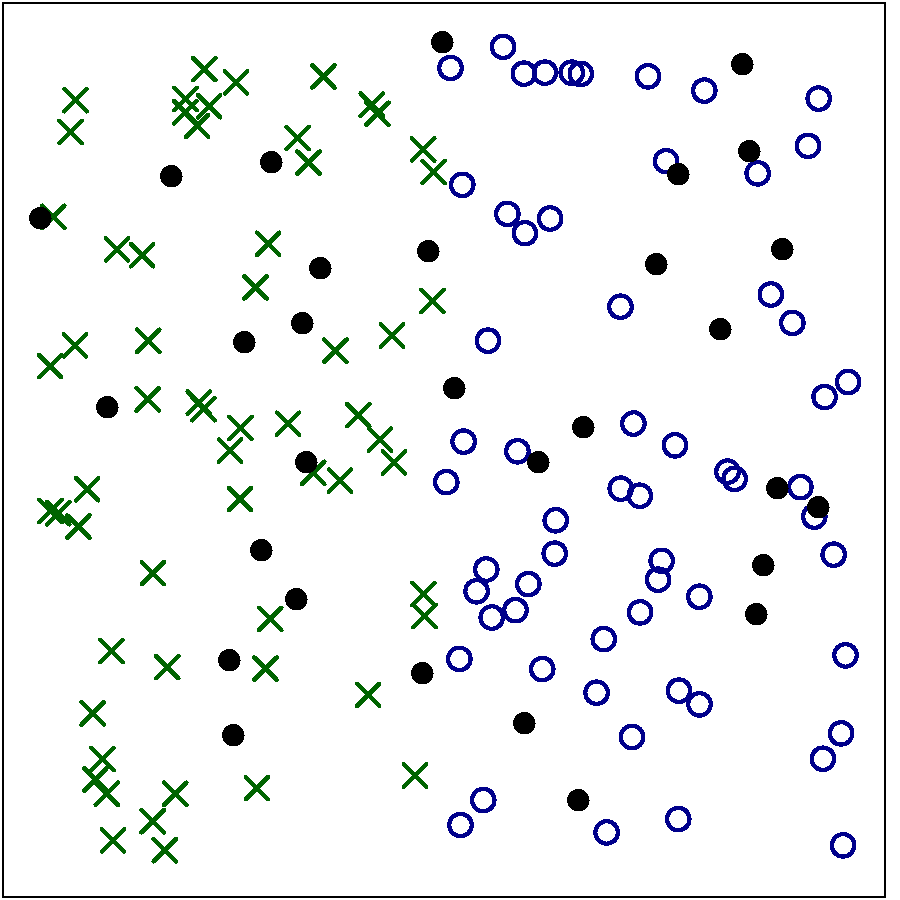
\includegraphics[width=0.45\textwidth]{inputs/img/chap1_scatter_intro_ds1} &
				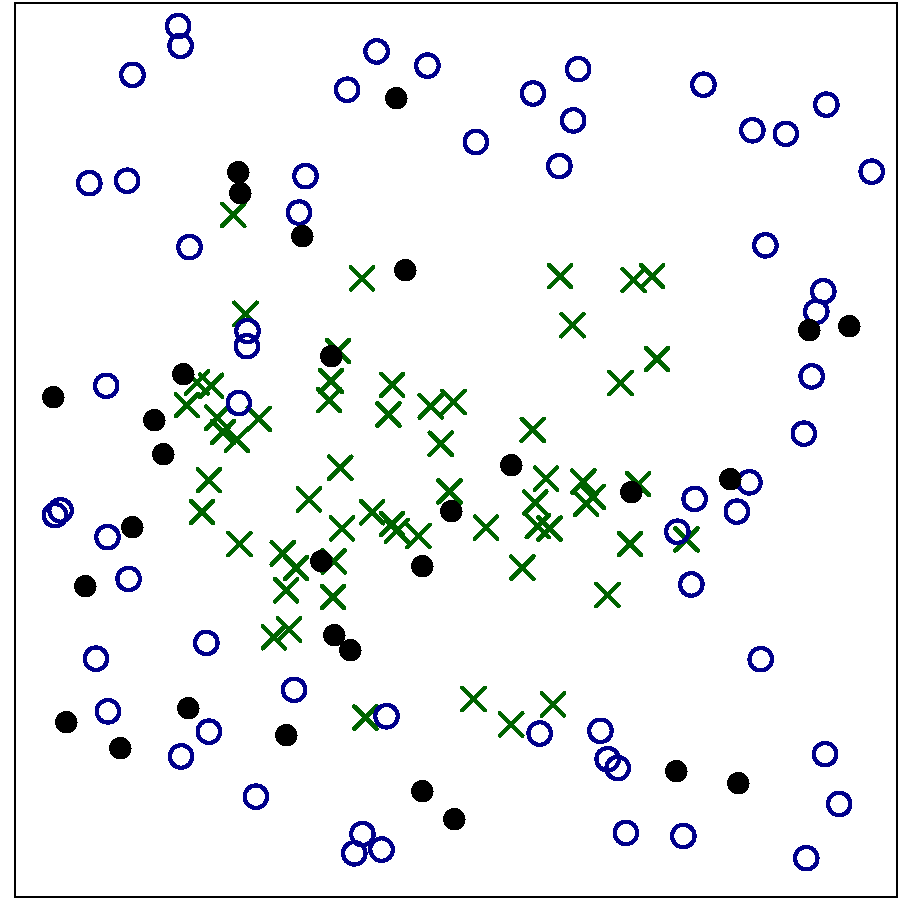
\includegraphics[width=0.45\textwidth]{inputs/img/chap1_scatter_intro_ds2} \\
			\end{tabular}
			\caption{Two classification examples in two dimensions. There are two known classes, asterisks and x marks. The problem is to classify the the unknown data, black bullets, into one of the two classes.}
		  	\label{fig:chap1_scatters}
		\end{figure}


	\section{Probabilistic model for data.}

		In this section we present our basic model. 
		
		In general, we define the law of $(X{\times}Y)$ as

		\begin{equation}
			(X,Y) \sim \mathbb{P}.
			\label{x_y_law}
		\end{equation}

		Assuming $x \in \mathcal{X}$, we can state that,

		\begin{equation}
			\mathcal{X} = \mathcal{R}^d.
			\label{x_example}
		\end{equation}

		where observations are represented by $d$-dimensional vector $x$. 

		In supervised learning, $y$ exists. It denotes the unknown nature of the observation, 
		and its characteristics depends on the classification problem. For instance,

		\begin{itemize}
			\item $|y|=2$, a binary problem, e.g. $Y = \{0,1\} \mbox{ or } \{-1,1\}.$;
			\item $|y|=K$, classification in a finite set of size K ;
			\item $y \doteq \mathbb{R}$, regression;
			\item $y = \mathbb{R}^K$, multi-task;
			\item $|y| = K$ observing the relative ordering between different values of $y$, ordinal regression.
		\end{itemize}
		
		\subsection{Definition of the law of $\mathbb{P}$.}

			We present two definitions of $\mathbb{P}$:

			\begin{enumerate}[a)] % a), b), c), ...
				\item Generative definition.
					\begin{equation}
						\mathcal{L}(X,Y) \equiv \mathbb{P} \leftrightarrow (\mathcal{Y}(Y), \mathcal{Y}(X|Y)).
						\label{p_generative_law_example}
					\end{equation}
				e.g. for $y=\{-1,+1\}$\\ 
				\centerline{$\mathcal{L}(X|Y) \leadsto (\mathbb{P}_{+},\mathbb{P}_{-})$}

				considering $\mathcal{L}(X|Y) \leadsto \mathcal{L}(X)$, and $(\mathbb{P}_{+},\mathbb{P}_{-}) \leadsto \mathcal{Y}(X|Y_{=+1})$, we have\\ 
				\centerline{$\mathbb{P}_X = _{P}\mathbb{P}_{+} + _{1-P}\mathbb{P}_{-}$}


				\item Alternative definition through a \emph{posteriori probability} function \cite{tc_Lugosi} (so-called ``dissertatif'' in french).
					\begin{equation}
						\mathcal{Y}(X,Y) \equiv (\mathcal{L}(X)\mathcal{L}(Y|X)).
						\label{p_generative_law_example}
					\end{equation}
			\end{enumerate}
			so that\\
			\centerline{$\forall x \in, \eta(x)=\mathbb{P}(Y=1|X=-1)$}
			Here, $\eta(x)$ represents the state of $X$.
		


	\section{Prediction problem statement.}
		
		\subsection{Types Prediction problems.}
			Based on the learning scenario, we can list predictions problems as follows:
	
			\begin{itemize}
				\item Classification: 
					\begin{itemize}
						\item classification data: $|y|<+\infty$; 
						\item goal: predict a new $x$.
					\end{itemize}
				\item Scoring or bipartite raking: 
					\begin{itemize}
						\item classification data: $|y|<+\infty$; 
						\item goal: ordering a new bunch of $X$, $(x_1,x_2,\dots,x_m)$, taking into account the state of $x$, where $\eta(x)=\mathbb{P}(Y=1|X=x)$. An remarkable example of this kind of problem is the ranking mechanism of search engines.
					\end{itemize}
				\item Raking: 
					\begin{itemize}
						\item data features: e.g. $|y|=\{1,2,3\}$, where $1 \ll 2 \ll 3$;
						\item goal: ordering a new bunch $x$.
					\end{itemize}
				\item Preference learning: 
					\begin{itemize}
							\item $(X,X')$, and $sign(y-y')$
						\item goal: binary classification $(X,X'_Z)$, where $Z \in \{-1,1\}$.
					\end{itemize}
			\end{itemize}

		\subsection{How to approach a prediction problem.}
			\begin{itemize}
				\item Define the performance goal $R$. 
				\item Select the set of predictors $\mathcal{F}$. Examples: 
					\begin{itemize}
							\item Binary classification: $\mathnormal{f}:\mathbb{R}^d\rightarrow\{-1,1\}$
							\item Scoring: $\mathnormal{f}:\mathbb{R}^d \times \dots \times \mathbb{R}^d \rightarrow {\sigma}_m $ (permutation  of $m$ elements/vectors);
							\item Preference function: $\mathnormal{f}:\mathbb{R}^d \times \mathbb{R}^d \rightarrow \{-1,1\} \mbox{ or } \{-1,0,1\}.$
					\end{itemize}
			\end{itemize}

		\subsection{Performance/error issues.}

			Lets define

			\[ \forall x \in, \mathnormal{f}, R(f)=\mathbb{E}[l(Y,f(x))] =  \int_{x{\times}y} f(x)\,dP(x,y).\] 

			where $l:y{\times}y \rightarrow \mathbb{R}^d$ is the measure of \emph{loss} or \emph{error}.
			
			Examples of loss:
					\begin{itemize}
							\item Binary classification: $l(y,f(x)) = 1|\{y \neq f(x)\}$.
							\item Regression: $l(y,f(x))=(y_f(x))^2$.
							\item Optimization issue: $l(y,f(x))=(1-yf(x))_+ = \Phi(yf(x))$.
							\item Log likelihood: $l(f(x))=\ln(f(x))$.
					\end{itemize}

	\section{Example: supervised classification}
		%\subsection{} 

	\chapter{Classification algorithms.}

This chapter presents the classic classification methods, mostly for binary classification.

\emph{A generic problem formulation}: for Binary classification, $(X,Y)$, $Y \in \{0,1\}$  

\begin{itemize}
	\item Rules: $f : \mathbb{R}^d \rightarrow \{0, 1\}$
	\item Criteria: $R(f) = \mathds{1}_{Y \neq f(x)}$
	\item n-samples: $\mathcal{D}_n=\{(X_1,Y_i)\}, i\in\{1,\dots,n\}$
\end{itemize}


\emph{Notions of local averaging}:

\begin{itemize}
	\item notion of the neighbourhood of $x \in \mathbb{R}^d$ 
	\item Weighting (pondération de poids) among neighbours  
	\item Majority rule
\end{itemize}

Weighting $W_{ni}(X,\mathcal{D})$: decision made by the weighting majority
\[
	\hat{f_n}(x) = \left\{
			  \begin{array}{l l}
			    +1 & \quad \text{if } \sum_{i=1}^n W_{n,i}(X,\mathcal{D})\mathds{1}_{Y_i = +1} > \sum_{i=1}^n W_{n,i}(X,\mathcal{D})\mathds{1}_{Y_i = 0}\\
			    0 & \quad \text{otherwise.}\\
			  \end{array} \right.
\]
\[
	\hat{f_n}(x) = \mathds{1}_{\hat{{\eta}_n (x)>\frac{1}{2}}} \text{, where } \hat{{\eta}_n(x)}=\sum_{i=1}^n W_{n}(X,\mathcal{D})y_i.
\]



	\section{The nearest-neighbour case.}

		\emph{Definition}: consider $\mathcal{D}_n$ n-samples of type $(X,Y)$, $Y$ binary over $\{0,1\}$, the k-nearest neighbours (KNN) of $x$ in $\{X_1,X_2,\dots,X_n\}$ are given by the collection $\{X_{(1)}(x),X_{(2)}(x),\dots,X_{(k)}(x)\}=N_k(x)$, such as $\|X_{(1)}(x)-x\| \leq  \|X_{(2)}(x)-x\| \leq \dots \leq \|X_{(n)}(x)-x\|$. KNN requires a norm definition $\|\cdot
\|$.

		\emph{Definition}: k-nearest-neighbour prediction rule for classification.

		Assuming that $W_{n,i}(i=W_i(x,\mathcal{D}_n))$ are weights for 

			\[
			  x_i = \left\{
			  \begin{array}{l l}
			    \frac{1}{K} & \quad \text{if $x_i\in N_k(x)$;}\\
			    0 & \quad \text{otherwise.}\\
			  \end{array} \right.
			\]

		so that, the rule of KNN is given by

			\[
			  \forall x\in\mathbb{R}^d, \hat{f}_n = \left\{
			  \begin{array}{l l}
			    1 & \quad \text{if $\sum_{i=1} W_{n,i}, \mathds{1}_{Y_i=+1}>\sum_{i=1}^{n} W_{n,i}\mathds{1}_{X_i=0}$;}\\
			    0 & \quad \text{otherwise.}\\
			  \end{array} \right.
			\]

		This definition raises important questions, such as:

		\begin{itemize}
			\item which norm $\|\cdot\|$ to choose?
			\item what k? fixed or in function of n
			\item and the weights, should they be uniform distributed or not?
		\end{itemize}


	\section{The averaging principle.}

		\subsection{Plug-in} 
			$\mathcal{D}_n=\{(X_1,Y_i)\}, i\in\{1,\dots,n\}$

			\[
			  \hat{f}_n(x)=sgn(\hat{\eta}(x)=\sum_{i=1}^{n} W_{n,i}Y_i
			\]
			
			where $(W_{i,n})_{1\leq i\leq n}$ are convex weights.
		
		\subsection{Examples} 
					\begin{itemize}
						\item KNN (as homework)
						\item partitions
							Considering $A_1,A_2,\dots$ a subset of $\mathbb{R}^d$? (composing a partition $U_j A_j=\mathbb{R}^d$ and $\mu(A_i\cap A_j)=0$ if $i\neq j$)
							\[
							  W_{ni}(x)=\frac{\mathds{1}_{x_i\in A(x)}}{\sum_{j=1}^{n} \mathds{1}_{x_{i\in A(x)}}}
							\]
							where $A(x)=\{A_k;x\in A_k\}$

							
						\item kernel, $k:\mathbb{R}^d\rightarrow\mathbb{R}_+$ 

							assuming a window $h>0$
							\[
							  W_{hi}(x)=\frac{k(\frac{x_i-x}{h})}{\sum_{j=1}^{n} k(\frac{x_i-x}{h})}
							\]

							
					\end{itemize}


	\section{The plug-in rule.}

		Given $\eta(x)=\mathbb{P}(Y=1|X=x) \forall x \in \mathbb{R}^d$.

		\textbf{Definition}:  If $\hat{\eta}$ a function that estimates $\eta$ so that related plug-in rule is $\hat{f} = \mathds{1}_{\{\hat{\eta\}}> \frac{1}{2}}$.

		\emph{Justification}: optimal rule $f^* = \mathds{1}_{\{\eta> \frac{1}{2}\}}$  

		\emph{Proposition}: If $\hat{f_n}(x) = \hat{f_n}(x,\mathcal{D}) = \mathds{1}_{\{\hat{{\eta}_n}\}(x)>\frac{1}{2}}$ , then,
		\[
			\mathbb{E}_{\mathbb{P}\otimes n}R(\hat{f_n} - R({f^*}) \leq 2\mathbb{E}_{\mathbb{P}\otimes n\otimes\mathbb{P}_x}[|\hat{{\eta}_n}(x) - {\eta}(x)|]
		\]

		\textbf{Proof}:

		We have seen that 
		\[
			\forall f\text{,} R(f^*) \leq 2\mathbb{E}[|\eta(x)-\frac{1}{2}|\mathds{1}_{\{f(x)\neq f(x)\}}]
		\]
		conditioning $\mathcal{D}_n$, from where
		\[
			R(\hat{f_n}) - R({f_*}) \leq \leq 2\mathbb{E}[|\eta(x)-\frac{1}{2}|\mathds{1}_{\{f^*\neq \hat{f_n}\}}]
		\]
		since $\{f^*\neq \hat{f_n}\}$, we have $|\eta - \frac{1}{2}|\leq|\eta - \hat{{\eta}_n}|$, in other words, we can ensure the convergence.

		\textbf{Begin of Note}

		\emph{Remarks}: Classical plug-in rules
					\begin{itemize}
						\item Linear discriminant analysis		
						\item Logistic linear regression		
					\end{itemize}

		These classical plug-in rules are deprecated, at least for classification. They make a Gaussian hypothesis, that means a linear separating.

		\emph{Exercise}: Given $\mathbb{E}|\hat{{\eta}_n} - \eta(x)|  \xrightarrow[n\to \infty]{} 0$, so that $\frac{\mathbb{E}R(\hat{f_n})-R(f^*)}{\sqrt{\mathbb{E}|\hat{{\eta}_n}-\eta(x)|^2}} \xrightarrow[n\to \infty]{} 0$
		
		\emph{Remarks} (very important): It is much mode difficult  estimate $\eta$ than identify classes/groups of a classification problem.

		\emph{Remarks}: Audibert-Tsybakov [AoS'11]: High speedy for plug-in rules following the hypothesis of regularity over the borders of ensembles  of $\eta$ plus conditional margin.

		Condition of margin (CM) [Tsyb.'04]

		Hypothesis: $\exists c > 0$, $\exists \alpha \geq 0$, such as $\operatorname{P}_x(0<|\eta - \frac{1}{2}|<t)\leq ct^{\alpha}$, $\forall t$. 

		Special cases:
		\begin{itemize}
			\item $\alpha = 0 \to	c$, a trivial case, CM is not required	
			\item $\alpha = +\infty \to \exists \delta : |\eta(x) - \frac{1}{2}| > \delta$, $\forall x$, that means that exists a border/margin where there is no ambiguity. 		
		\end{itemize}

		Results over CM:
		  \begin{align*}
            \mathbb{E}(R(\hat{f_n})-R(f^*)) &\leq 2c\mathbb{E}[\|\hat{{\eta}_n - \eta}\|^{1+\alpha}_{\infty}]\\
						 &\leq c_1(\alpha,p)\mathbb{E}\|\hat{{\eta}_n}-\eta\|^{\frac{p(1+\alpha)}{p+\alpha}}_{p}, \forall p \geq 1, \alpha > 0
		  \end{align*}

		\emph{Remarks}:  If $R(f^*)=0$ (no noise), then $\mathbb{E}R(\hat{{\eta}_n})\leq 4\mathbb{E}[|\hat{{\eta}_n}(x)-\eta(x)|^2]$, $\eta(x)\in\{0,1\}$

		\textbf{End of Note}


	\section{Consistency analysis.}
		
		This section describes the universal consistence of methods based on local averaging.

		Recall: week universal consistency $\forall \operatorname{P}$, $R(\hat{f_n}) - R(f^*) \xrightarrow[n\to \infty]{\operatorname{P}} 0$ (week consistency, it means consistency through probability)

		\emph{Remark}: $W_{nj}$ weight depends on the sample locations.

		\textbf{Theorem}(stone):

		Suppose (hypothesis)
		\begin{enumerate}
			\item Regularity
				$\exists c>0 such as$
				\[
					\forall \text{measurable} f : \mathbb{R}^d \to \mathbb{R}_+ \text{such as} \mathbb{E}(f(X)) < +\infty
				\]
				so that
				\[
					\mathbb{E}[\sum_{j=1}^{n} W_{n,j}(X,\mathcal{D}_n)f(X_j)] \leq c\mathbb{E}(x)
				\]
			\item Border/limits 
				\[
					\forall a > 0, \lim_{x \to \infty} \mathbb{E}(\sum_{j=1}^{n} W_{n,j}(X,\mathcal{D}_n)\mathds{1}_{\{\|X-X_j\|\leq a\}}) = 0 
				\]
			\item Weight distribution 
				\[
					\lim_{n \to \infty} \mathbb{E}[\underset{1\leq j \leq n}{\operatorname{max}} W_{nj}(X,\mathcal{D}_n)] = 0 
				\]

		\end{enumerate}
		
		So that, we have $R(\hat{f_n})  \xrightarrow[n\to \infty]{\operatorname{P}} R(f^*)$ for $\hat{f_n} = \mathds{1}_{\{\text{... lost }\}}$ 

		\textbf{Proof}:

			It just requires to show that

			\[
				\| \hat{{\eta}_n} - \eta \| = \mathbb{E}(\hat{{\eta}_n} - \eta)^2 \xrightarrow[n\to \infty]{} 0, \text{that means, it is small.}
			\]

			\emph{hypothesis}:

			\begin{itemize}
				\item given $\overline{\eta}(X,\mathcal{D}_n) = \sum_{j=1}^{n} W_{n,j} (X,\mathcal{D}_n) \eta(x_j)$
				\item $\| \eta - \hat{\eta} \| \leq \underbrace{\| \eta - \overline{\eta}_n \|}_{\mathrm{(I)}} + \underbrace{\| \overline{\eta}_n - \hat{\eta}_n \|}_{\mathrm{(II)}}$
			\end{itemize}
			
			\begin{enumerate}[1.]%for capital roman numbers.
				\item putting $\mathrm{(I)}$ under control: 

					$\forall x, ( \eta(x) - \overline{\eta}_n )^2 = (\sum_{j=1}^{n} W_{n,j}(x)( \eta(x) - \eta(x_j)))^2 \leq \sum_{j=1}^{n} W_{n,j}(x)( \eta(x) - \eta(x_j))^2 $, convex weight adjustment through convexity inequality (according to Jensen)
					
					\emph{Remark} (about Jensen principle): $f({\alpha}x + (1 - \alpha)y) \leq {\alpha}f(x) + (1 - \alpha)f(y), f$ convex, $\alpha \in [0,1]$ 

					There are two particular cases:
	
					\begin{enumerate}[(a)]
						\item $\eta$ is $\text{unif.}^\pm C^0$

							$\forall \varepsilon > 0, \exists a > 0$ such as (suppose) $| \eta(x_1) - \eta(x_2) | < \varepsilon, x_1, x_2; \|x_1 - x_2\| \leq a$

							By the integral 

						  \begin{align*}
				            \| \eta - \overline{\eta}_n\|^2  & \leq \mathbb{E}[ \sum_{j=1}^{n} (\mathds{1}_{\{\|x - x_j\| \leq a\}} + \\
										 & \mathds{1}_{\{\|x - x_j\| > a\}})W_{n,j}(x)( \eta(x) - \eta(x_j))^2 ]\\
										 & \leq \varepsilon + \mathbb{E}(\sum_{j=1}^{n}W_{n,j}(x)\mathds{1}_{\{\|x - x_j\| > a\}})
						  \end{align*}

						Which means uniform continuity and convex weights. When $W_{nj} \to 0, n \to \infty $ (hypothesis 2), $|\eta(x_1) - \eta(x_2)| \leq 1, \forall x_1, x_2$.
							
						\item $\eta$ is not Unif. $\pm c^0$: we consider continuous density functions with compact support in $L^2(\mathbb{P}_x), \forall \varepsilon > 0, \exists \tilde{\eta} \text{unif.}^\pm C^0 $ such as $\|\eta - \tilde{\eta}\| \leq {\varepsilon}L^2(\mathbb{P}_x)$. We have $\tilde{{\eta}_n}(X,\mathcal{D}_n) = \sum_{j=1}^{n}W_{n,j}(X,\mathcal{D}_n)\tilde{\eta}(x_j)$. So that, $\|\eta - \overline{\eta}\| \leq \underbrace{\|\eta - \tilde{\eta}\|}_{ \leq \varepsilon \text{(density)}} + \underbrace{ \|\tilde{\eta} - \tilde{{\eta}_n}\|}_{\text{case a)}} + \|\tilde{{\eta}_n} - \overline{\eta}\| $

						so that,
			
						\[
							\|\hat{{\eta}_n} - \overline{\eta} \|^2 = \mathbb{E}[(\sum_{j=1}^{n}W_{n,j}(x)(\tilde{\eta}(x_j) - \eta(x_j)))^2]
						\]

						applying Jensen,

						  \begin{align*}
				            \|\hat{{\eta}_n} - \overline{\eta} \|^2  & \leq \mathbb{E}[\sum_{j=1}^{n}W_{n,j}(x)(\tilde{\eta}(x_j) - \eta(x_j))^2] \\
										 & \leq c\mathbb{E}[(\tilde{\eta}(x) - \eta(x))^2] \\
										 & \underbrace{\leq}_{\text{hypothesis 1 with} f = (\tilde{\eta} - \eta)^2} c{\varepsilon}^2 \text{(continuous uniform)}
						  \end{align*}

					\end{enumerate}
					
				\item putting $\mathrm{(II)}$ under control $\|\hat{\eta} - \overline{\eta} \|^2 \leq \mathbb{E}[\sum_{j=1}^{n}W_{n,j}(x)({\eta}(x_j) - y_j)]^2$ : 

						  \begin{align*}
				            \mathbb{E}[\sum_{j=1}^{n}W_{n,j}(x)({\eta}(x_j) - y_j)]^2  &  \\
										 & = \mathbb{E}[\sum_{j=1}^{n}W_{n,j}^2(x)(\tilde{\eta}(x_j) - y_j)] + \underbrace{(\text{double products})}_{= 0}\\
										 & \leq \mathbb{E}[\sum_{j=1}^{n}W_{n,j}^2(x)] \\
										 & \leq \mathbb{E}[\underset{1\leq j \leq n}{\operatorname{max}} W_{n,j}(x)] \underbrace{\xrightarrow[n\to \infty]{}}_{\text{hypothesis 3}} 0
						  \end{align*}

							because $\eta(x) = \mathbb{E}(Y|X=x)$ and $(x_i,y_i) \sqcup (x_j,y_j), \forall i \neq j$.

			\end{enumerate}

		\textbf{Corollary} (there are enough proven conditions for universal consistency)

			\begin{enumerate}[(a)]
				\item Partition
					
						Given $A_{1,n}, A_{2,n}, \dots, $ followed by a uncountable number of partitions, have to follow two conditions:
						
						\begin{itemize}
							\item $\forall r \lim_{n \to \infty} \frac{\operatorname{cardinality of \{k \in \mathbb{N}: A_{k,n} \cap B(0,r)\}}}{n} = 0$, where B stands for bubble.
							\item $\lim_{n \to \infty} \underset{k}{\operatorname{max}} \{diameter(A_{k,n})\} = 0$.
						\end{itemize}

						Special case: regular grid of $h=h_n$ over $\mathbb{R}^d$, $h_n \xrightarrow[n\to \infty]{} 0 $ and $nh_n^d \to +\infty$.

				\item Kernel: kernel k (positive function, with a $h>0$ window limit/border)

					Condition: $\exists r, R_i 0<r<R<+\infty; \exists b > 0 $ such as $b z/B(0,r) \leq k \leq 1/B(0,R); h=h_n$ such as $h\to 0, nh_n^d \to +\infty$.

				\item K-NN
					
					$k=k_n$ such as $k_n \to +\infty; \frac{k_n}{n} \xrightarrow[n\to \infty]{} 0$

					\emph{Note}: $k$ must be neither too small nor too big.
			\end{enumerate}

			

	\section{Other rules/questions/practical aspects.}
		
			\emph{Exercises}:

			\begin{enumerate}[1.]
				\item find the algorithm complexity for K-NN.
				\item What happens if we add a new data?
			\end{enumerate}

			\emph{Best practices/practical aspects}:

			\begin{itemize}
				\item how to choose a partition/ partitioning: bast method is CART (easy to interpret), this highly efficient method empirically constructs partitions based on recursive tree structures.
				\item How to choose k, n, (complexity parameter): method of cross-validation: data is divided in V n-data packets (for test and learn, consider V equal to 5 packets, so that 4 for test, and 1 for test) of choose the best k, smallest error on average, changing $|V|$. (best practices shows that those packets might be between 5 and 10).
			\end{itemize}

%\subsection{} 

	\chapter{Inferential theory and statistical basis of learning.}

	%\section{}
		%\subsection{} 

	\chapter{Measure of complexity, penalization, and modelling.}

	%\section{}
		%\subsection{} 

	\chapter{The principles of aggregation of classifiers, predictors, and meta-algorithms}

	%\section{}
		%\subsection{} 


	\appendix

\chapter{Course organization and scheduling.}

		\section{Classes.}
			\begin{itemize}
				\item 10 class sessions;
				\item two hands-on sessions (TD): mid-October, and early December.
			\end{itemize}

		\section{Exams and gradings.}
			\begin{itemize}
				\item required mid-term written exam: by the end of December;
				\item final exam: (i) written exam by mid-December, or (ii) Mini-project, including a 20-pages report, and presentation early January.
				\item Bonus: (i) up to two points for hands-on sessions (TD) problem sheets solved, (ii) up to three points for writing down lecture notes.
			\end{itemize}

		\section{References.}
			\begin{itemize}
				\item Theory of Classification: a Survey of Recent Advances by Boucheron et. al.\cite{tc_Lugosi};
				\item A Probabilistic Theory of Pattern Recognition by Devroye et. al. \cite{ptpr}.
			\end{itemize}


	\bibliographystyle{plain}
	\bibliography{inputs/biblio.bib}

\end{document}